\section{Kanal-Codierung}\label{sec:kanal-codierung}

\subsection{Fehlerkorrektur}\label{subsec:fehlerkorrektur}

\begin{definition}{Kanalcodierungstheorem von Shannon}
    Man kann über einen diskreten gedächtnislosen Kanal (DMC) mit der Coderate $R$ fehlerfrei übertragen, so lange $R$ nicht grösser ist als die Kanalkapazität.
    Möchte man die Restfehlerwahrscheinlichkeit eines Fehlerschutzcodes beliebig klein machen, so muss $R < C$ sein.
    Hierbei ist $C$ die Kanalkapazität in bit/bit (Nutzbare Bits pro Kanalbenutzung) \[C_{\text{BSC}}(\epsilon) = 1 - H_b(\epsilon)\] und $R$ die Coderate in bit/bit (Infobits pro Codebit) \[R = \frac{K}{N},\] wobei $K$ die Länge der Infowörter und $N$ die Länge der Codewörter ist.
    $R$ muss kleiner als $C$ sein, damit alle Informationen in den nutzbaren Bits Platz hat.
\end{definition}

\subsection{Binäre symmetrische Kanäle}\label{subsec:binaere-symmetrische-kanaele}

Bei einem symmetrischen binären Kanal (engl.\ Binary Symmetric Channel, BSC) gilt:
\begin{itemize}
    \item Die Fehlerwahrscheinlichkeit $\epsilon$ ist unabhängig vom Eingangssymbol.
    \item Die Wahrscheinlichkeiten $P(y_m \mid x_n)$ der Übergänge (bei gegebenem $x_n$) sind:
    \begin{center}
        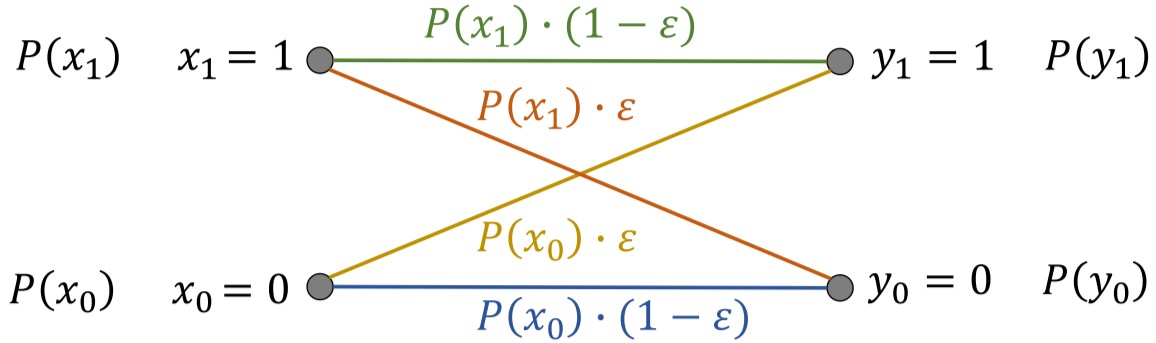
\includegraphics[scale=0.25]{binary-symmetric-channel}
    \end{center}
\end{itemize}

\subsubsection{Bitfehlerwahrscheinlichkeit}

Die \emph{Bitfehlerwahrscheinlichkeit} $\epsilon$ (engl.\ Bit Error Ratio, BER) ist eine Eigenschaft des Kanals, die die Anzahl der fehlerhaften Bits im Verhältnis zur Gesamtzahl der Bits angibt.
Beispiele:
\begin{multicols}{2}
    \begin{itemize}
        \item Alle Bits falsch: BER = 1
        \item Kein Bit falsch: BER = 0
        \item 1 von 2 Bits falsch: BER = 0.5
        \item 1 von 1000 Bits falsch: BER = 0.001
    \end{itemize}
\end{multicols}

\subsubsection{Mehr-Bit-Fehlerwahrscheinlichkeiten}

\begin{definition}{Binomialkoeffizient}
    $\binom{n}{k}$ ist der $k$-te Koeffizient der Potenz des Binoms $(x + y)^n$.
    Es gilt mit $k \leq n$: $\binom{n}{k} = \frac{n!}{k! \cdot (n-k)!}.$
\end{definition}

\begin{definition}{}
    Die Wahrscheinlichkeit $P_{F,N}$, dass in einer Sequenz von $N$ Datenbits \emph{genau $F$ Bitfehler} auftreten, ist gegeben durch \[P_{F,N} = \binom{N}{F} \cdot \epsilon^F \cdot (1 - \epsilon)^{N-F},\] wobei der Binomialkoeffizient die Anzahl der Möglichkeiten angibt, $F$ Fehler in $N$ Bits anzuordnen. $\epsilon^F$ ist die Wahrscheinlichkeit für einen $F$-fachen Bit-Fehler, und $(1 - \epsilon)^{N-F}$ ist die Wahrscheinlichkeit, dass die restlichen $N-F$ Bits alle keinen Fehler haben.
\end{definition}

Für die Wahrscheinlichkeit, dass \emph{maximal $F$ Fehler} bei einer Übertragung von $N$ Bits auftreten, bilden wir die Summe aller Fälle: \[P_{\leq F,N} = \sum_{t=0}^{F} \binom{N}{t} \cdot \epsilon^t \cdot (1 - \epsilon)^{N-t}\]
Oft will man die Restfehlerwahrscheinlichkeit wissen, also die Wahrscheinlichkeit, dass \emph{mehr als $F$ Fehler} bei einer Übertragung von $N$ Bits auftreten: \[P_{\geq F,N} = \sum_{t=F+1}^{N} \binom{N}{t} \cdot \epsilon^t \cdot (1-\epsilon)^{N-t}\]

\subsubsection{Kanalkapazität}

Die maximale Kanalkapazität entspricht dem Maximum der Entropie einer binären Quelle: 1 Bit/Symbol = 1 bit/bit.
Die Störquelle kann ebenfalls als Binary Memoryless Source mit den Wahrscheinlichkeiten $\epsilon$ (Fehler) und $1-\epsilon$ (kein Fehler) betrachtet werden. \[C_{\text{BSC}}(\epsilon) = 1 - H_b(\epsilon) \\
= 1 - \left\{ \epsilon \cdot \log_2 \frac{1}{\epsilon} + (1-\epsilon) \cdot \log_2 \frac{1}{1-\epsilon}\right\}\]

\subsubsection{Hamming-Distanz}

\begin{definition}{Hamming-Distanz}
    Die \emph{Hamming-Distanz} ist die Anzahl der wechselnden Bits von einem gültigen Code zum nächsten gültigen Code
\end{definition}

Die Hamming-Distanz $d$ zwischen den Codewörtern ist nicht per se konstant:
\begin{multicols}{3}
    \begin{itemize}
        \item \texttt{d(00000, 01011) = 3}
        \item \texttt{d(01011, 10101) = 4}
        \item \texttt{d(00000, 10101) = 3}
        \item \texttt{d(01011, 11110) = 3}
        \item \texttt{d(00000, 11110) = 4}
        \item \texttt{d(10101, 11110) = 3}
    \end{itemize}
\end{multicols}

\begin{definition}{Minimale Hamming-Distanz}
    Für eine \emph{sichere} Fehlererkennung ist die minimale Hamming-Distanz $d_{\min}(C)$ eines Codes $C$ relevant: \[d_{\min}(C) = \min \limits_{j \neq k} d_H(c_j, c_k)\]
\end{definition}
Es lassen sich $d_{\min} - 1$ Bit-Fehler pro Codewort sicher erkennen und $\frac{d_{\min} - 1}{2}$ Fehler sicher korrigieren.
\begin{definition}{Hamming-Gewicht}
    Das \emph{Hamming-Gewicht} $w_H(c_j)$ gibt an, wie viele Einsen das Codewort $c_j$ enthält und darf nicht mit der Hamming-Distanz verwechselt werden!
    Sie wird verwendet, um die Hamming-Distanz zweier Codewörter zu bestimmen \[d_H(c_j,c_k) = w_H(c_j \oplus c_k)\]
\end{definition}

\textbf{Beispiele:}
\begin{multicols}{2}
    \begin{itemize}
        \item $w_H(000) = 0$
        \item $w_H(110) = w_H(011) = w_H(101) = 2$
        \item[]
    \end{itemize}
    \begin{itemize}
        \item $d_H(000,110) = w_H(000 \oplus 110) = w_H(110) = 2$
        \item $d_H(110,011) = w_H(110 \oplus 011) = w_H(101) = 2$
        \item $d_H(110,101) = w_H(110 \oplus 101) = w_H(011) = 2$
    \end{itemize}
\end{multicols}

\subsection{Binäre Blockcodes}\label{subsec:binaere-blockcodes}

\begin{itemize}
    \item \textbf{Systematik:} Die Informationsbits erscheinen im Codewort in einem Stück, ohne dass Fehlerschutzbits dazwischen vorhanden sind.
    Systematische Blockcodes sind einfach zu decodieren, da lediglich die Fehlerschutzbits entfernt werden müssen.
    \item \textbf{Linearität:} Bei einem linearen Blockcode ist die bitweise Exor-Verknüpfung von 2 Codewörtern wieder ein gültiges Codewort.
    Jeder lineare Code muss zwingend das Null-Codewort (000) enthalten.
    \item \textbf{Zyklizität:} Die zyklische Verschiebung eines Codeworts gibt wieder ein Codewort.
\end{itemize}

\subsection{Fehlererkennung}\label{subsec:fehlererkennung}

\subsubsection{Parität}

Eine einfache Methode für die Fehlererkennung macht Gebrauch eines \emph{Paritätsbit} (parity bit) über ein Datenbyte.
Hierbei setzen wir \emph{Even Parity}, wenn die Anzahl der Einsen inklusive Parity-Bit gerade ist, und \emph{Odd Parity}, wenn sie ungerade ist.
Beide sind gleichwertig, aber nur Even Parity ist linear.
\begin{center}
    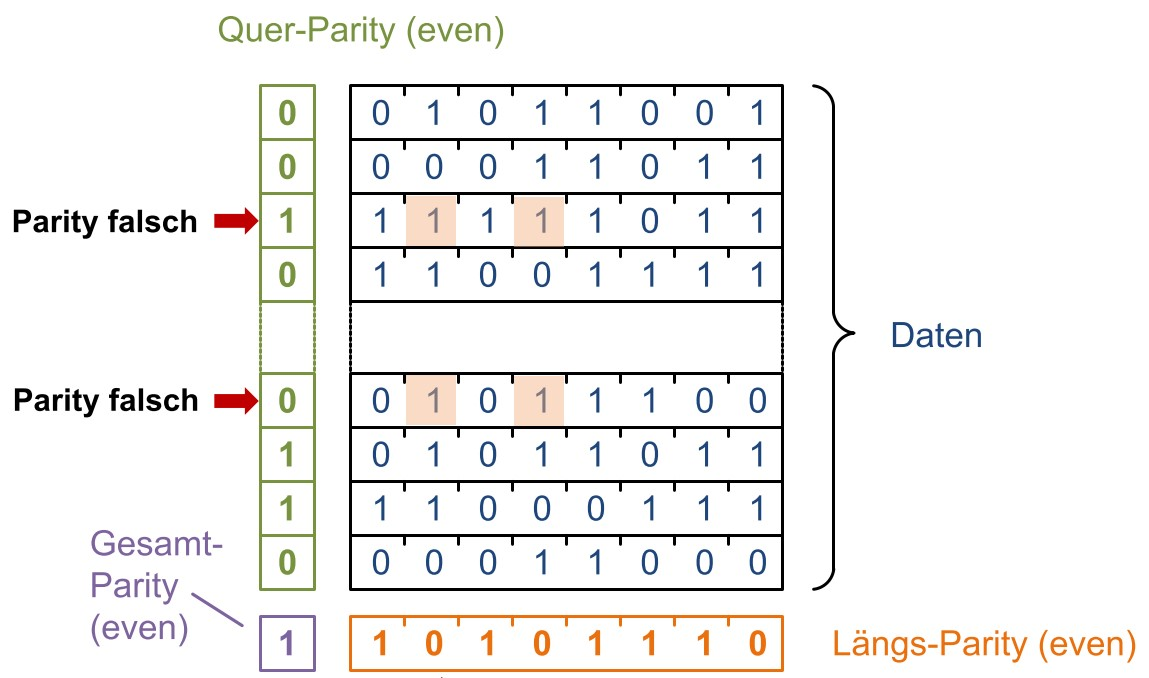
\includegraphics[scale=0.3]{parity}
\end{center}

\subsection{Fehlerkorrigierende Codes}\label{subsec:fehlerkorrigierende-codes}

\subsubsection{Hamming-Codes}

\begin{center}
    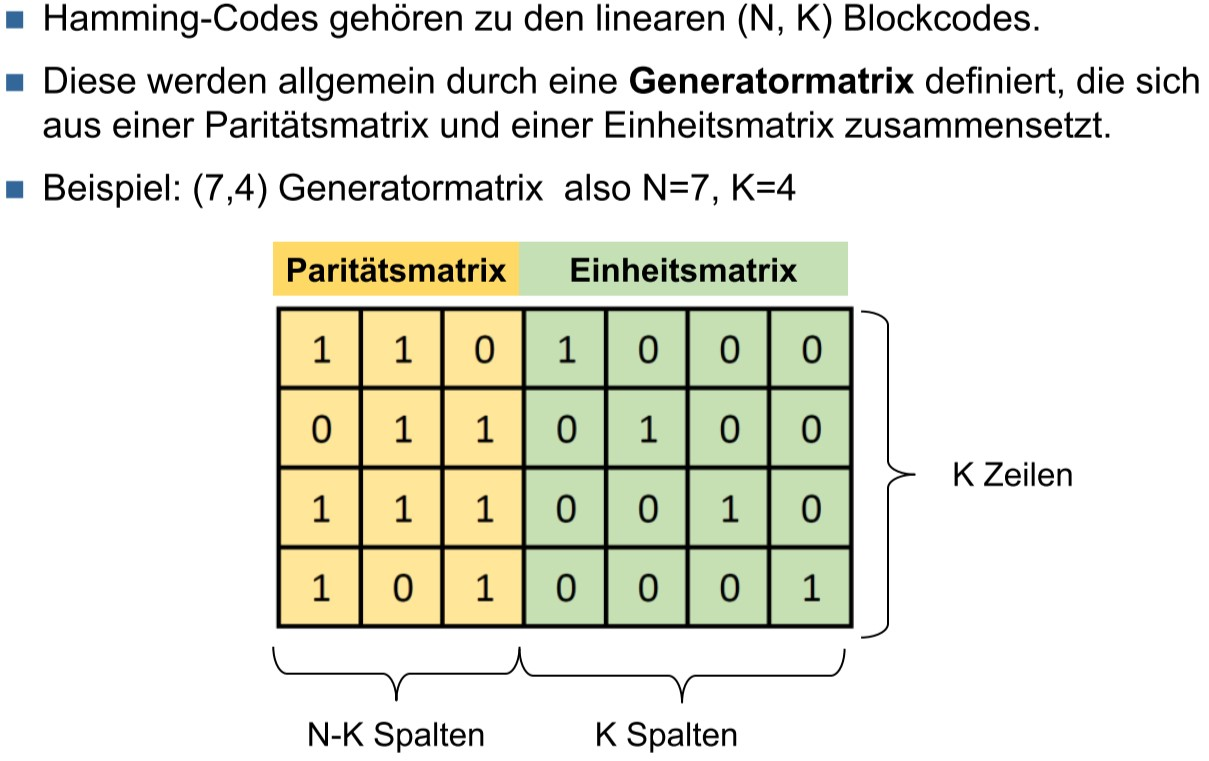
\includegraphics[scale=0.27]{generator-matrix}
    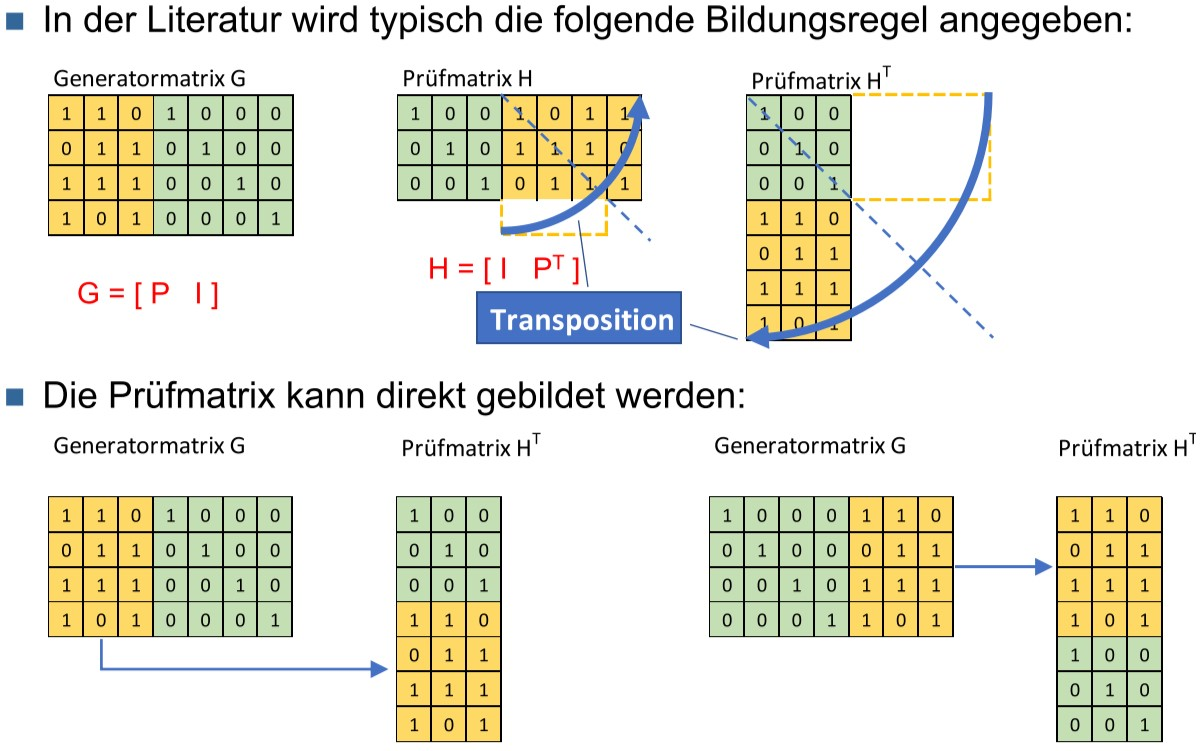
\includegraphics[scale=0.27]{pruef-matrix}
\end{center}

Hamming-Codes sind lineare Blockcodes unterschiedlicher Länge mit einer minimalen Hamming-Distanz von $d_{\min} = 3$.
Diese Codes sind optimal und demnach in der Lage 1-Bit Fehler sicher korrekt zu korrigieren.
2-Bit Fehler lassen sich sicher erkennen.

\subsubsection{Faltungscode}

\begin{definition}{Freie Distanz}
    Bei Faltungscodes spricht man nicht von minimaler Hamming-Distanz, sondern einer \emph{freien Distanz $d_{free}$}.
    Man wählt hierbei den kürzesten Weg von $00$ wieder zu $00$, wobei mind.\ eine 1 im Weg vorhanden sein soll (Zahl unter dem Strich).
\end{definition}

\begin{center}
    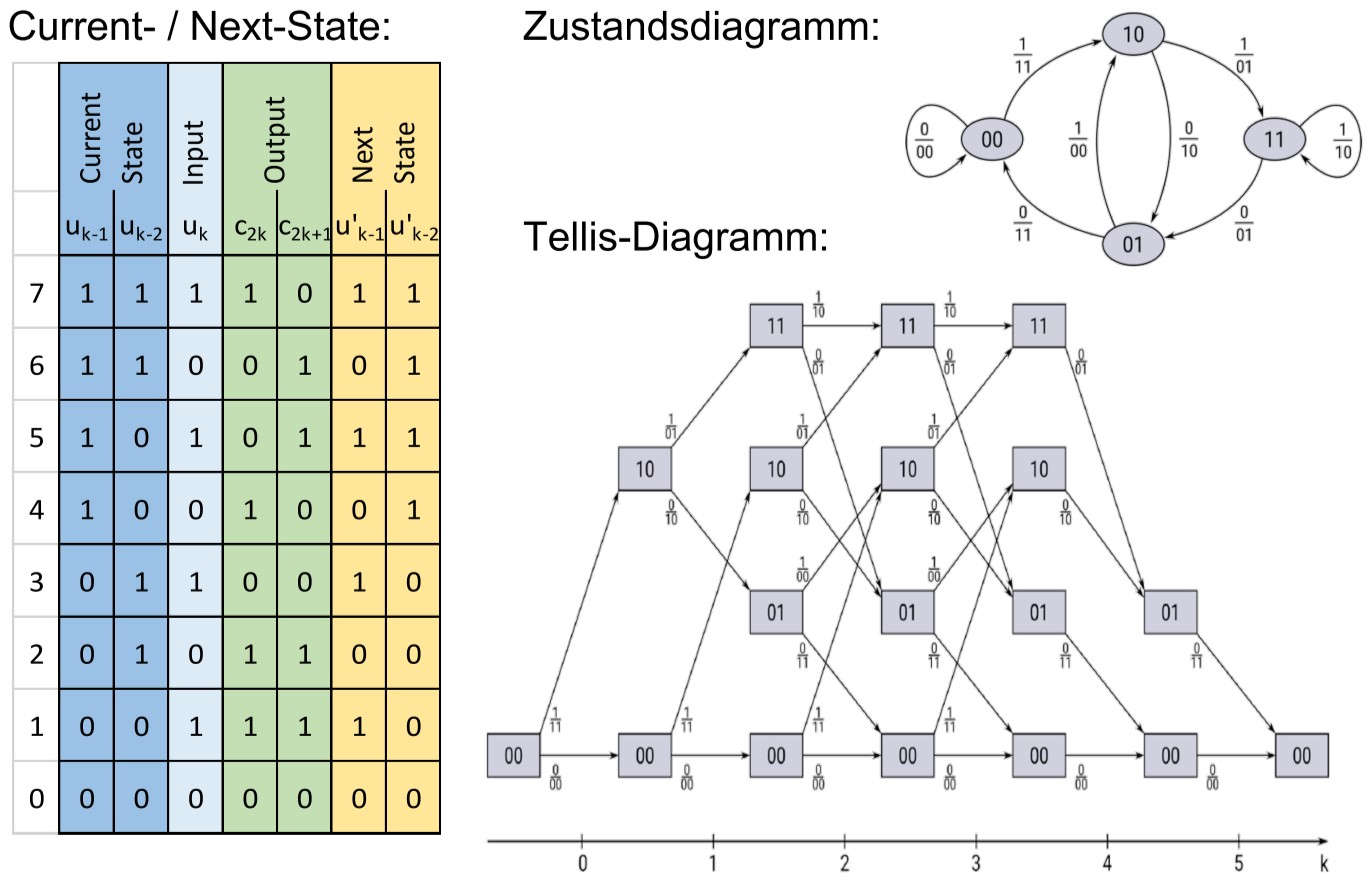
\includegraphics[scale=0.4]{trellis-diagramm}
\end{center}

\begin{center}
    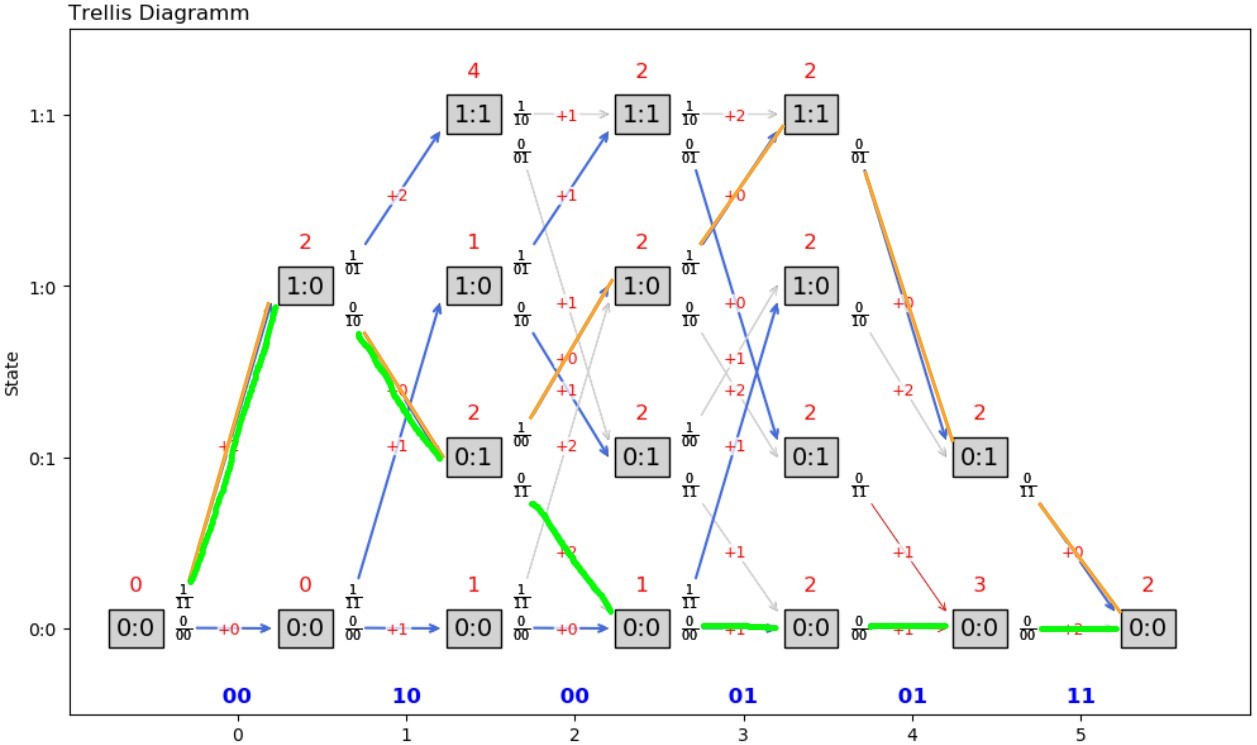
\includegraphics[scale=0.4]{trellis-diagram-example}
\end{center}